\begin{figure}
    \centering
    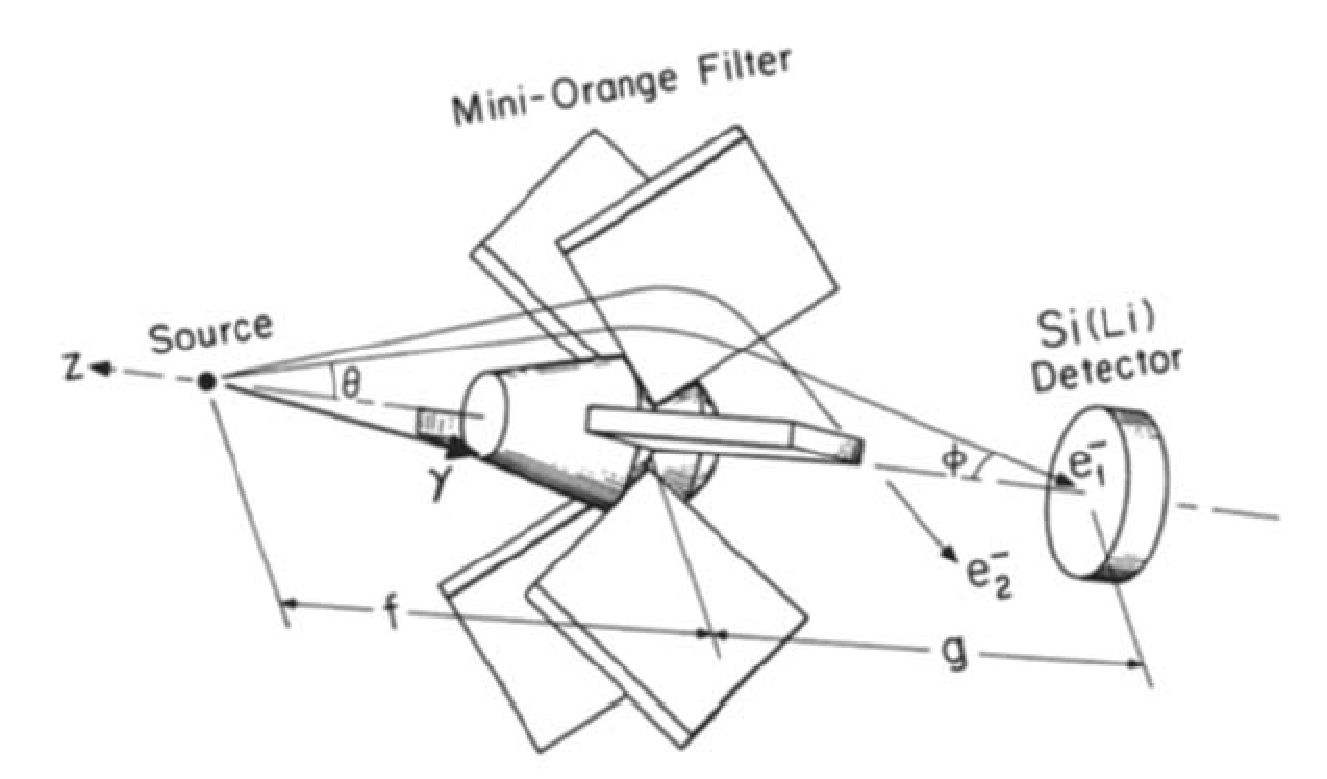
\includegraphics[scale=0.6]{Setup_Figs/mini-orange-metlay-figure.pdf}
    \caption{Graphic of the mini-orange filter. The central blocker keeps $\gamma$-rays from hitting the detector. The magnets bend electrons toward the detectors, and positrons away from the detectors. Being permanent magnets, they are optimized for a range of electron energies, and can cause overbending or underbending of electrons outside of that energy range, making the magnetic filter a factor in the efficiency. Taken from \citep{metlay93:_iceball_comm}}
    \label{fig:mini_orange}
\end{figure}